\section{Background}
Before introducing \sys, we will provide context to the problem.

\subsection{Motivating Example}
To understand how we can have non-trivial privacy constraints but still allow for data cleaning, consider the following scenario.
We are using an online application to collect course evaluations (e.g. M-CAFE \cite{zhou2015m}).In a simplified model, the data are collected in a relation $R$ with a categorical \textsf{major} attribute and one numerical \textsf{score} for the instructor (0-100):
\[
R(score,major)
\] 
Even though the data are anonymous, the relation $R$ is not private.
The instructor might be able to identify individuals with rare \textsf{major} values, and consequently, may penalize those who left a low score.

Now suppose we want to release the relation $R$ for analysis by the course instructors.
Let $M$ be the set of all majors, we can apply the following privacy mechanism: with probability $p$ replaces $r[score]$ with a random value from $M$. 
Intuitively, if the relation is large enough (we will formalize this precisely later), it is likely that by chance those rare demographics will be assigned to at least a few other students; affording some level of ambiguity.
From a data cleaning perspective, even though the individual records have been randomized, the domain is still preserved.
Errors that do not require record-level information can still be cleaned. 
For example, suppose \textsf{major} has alternative representations of the same logical value ``Electrical Engineering and Computer Sciences" and ``EECS".

It turns out that this is a little bit of an over-simplification, and to answer queries will require re-weighting results appropriately to account for the cleaning.
Furthermore, we will also have to apply randomization to the \textsf{score} attribute.
Consider the case when there is a very strong correlation between \textsf{major} and \textsf{score}, e.g., all Civil Engineering majors gave a \textsf{score} of 1. 
This can de-privatize our results, and we will discuss the solution to this problem in subsequent sections.
However, in this section, for ease of presentation, we will use this simplified model as a running example.

\subsection{Local Differential Privacy}
Local differential privacy is a measure of randomness in record-by-record transformations.
There is a parameter $\epsilon$, where larger values implies less randomness.
Let $R$ be a relation over the attributes $A$. A randomized algorithm
$M:R\mapsto\mathcal{D}$ is said to be $\epsilon$-local differentially
private if for all records $r,r'\in R$ and for any measurable subset
$S$ of the range of $M$:
\[
\sup_{r,r'}\frac{P[M(r)\in S\mid r]}{P[M(r')\in S\mid r']}\le\exp(\epsilon)
\]
In other words, given some observed randomized result $S$, $\epsilon$ is a bound on the ratio between the most likely input and the least likely input.

\noindent\textbf{Example of $\epsilon=0$: } This implies perfect privacy where observation of the private output does not make any input any more likely. An example of this would be an ideal one-way hash function.

\vspace{0.5em}

\noindent\textbf{Example of $\epsilon=\infty$: } Note that this does not imply no privacy. This only implies that observation of the private output excludes certain inputs. An example of this would be adding uniform random noise in $[-1,1]$ to numerical attributes. 

\begin{example}
Suppose a record $r$ from the course evaluation dataset has a \textsf{major} of ``Civil Engineering".
After applying the randomization, with probability $\approx 1-p$\footnote{The probability is not quite $1-p$, it is $1-p+p\frac{1}{N}$} the value stays the same ``Civil Engineering", else it is set to another value.
Due to symmetry $\epsilon = \ln \frac{1-p}{p}$.
\end{example}

\subsection{Database Model and Assumptions}
We formalize the intuition from the course evaluation example.
Let $R$ be a relation of a set of numerical attributes $A = \{a_1,...,a_k\}$, and a set of discrete valued attributes $D = \{d_1,...,d_l\}$.
We explore aggregate queries $f$ on this relation of the following form:
\begin{alltt}
SELECT \textsf{f}(a) FROM R WHERE cond(d)
\end{alltt}
where $a$ is a numerical attribute, and $d$ is a discrete attribute.

We consider data corruption in the discrete attributes of $R$.
In particular, there is a clean relation $R_{clean}$ (with the same schema as $R$) in which records have a one-to-one mapping with the dirty records.
This does not include record duplication errors or other types of schema errors.
We assume that these errors can be fixed using \emph{local} data cleaning operations (formalized subsequently).

\subsection{Local Cleaners}
We assume the existence of deterministic local data cleaning operations.
Let the set of discrete attributes $D$ be partitioned into $k$ subsets denoted by $g_i$:
\[
D = \cup_i^k g_i
\] 
Each \emph{local} cleaner $C_i(\cdot)$ is associated with a $g_i$, that is, given a record projected along $g_i$ it deterministically cleans the projection:
\[
g_i \subseteq D \text{ , } C_i : R[g_i] \mapsto R_{clean}[g_i]
\]
In other words, these cleaners can repair a discrete value only given local information, i.e., a subset of other attributes.
The cardinally of $g_i$ has implications on the granularity of privacy that is possible.
This is a restrictive assumption, but there are a number of common settings where such cleaners exist.

\begin{example}
Suppose \textsf{major} has alternative representations of the same logical value ``Electrical Engineering and Computer Sciences" and ``EECS". The find-and-replace operation ``Electrical Engineering and Computer Sciences -> EECS" is a local cleaner along the \textsf{major} attribute.
\end{example}

\begin{example}
Consider \textsf{major} values of ``Electrical Engineering and Computer Sciences" and ``Civil Engineering". The extract operation that finds the phrase ``Engineering" is a local cleaner along the \textsf{major} attribute.
\end{example}

\begin{example}
Suppose one student had \textsf{major} value of ``NULL". The value filling operation is \textbf{NOT} a local cleaner since it cannot be fixed given the information in the relation.
\end{example}

\begin{figure}[t]
\centering
 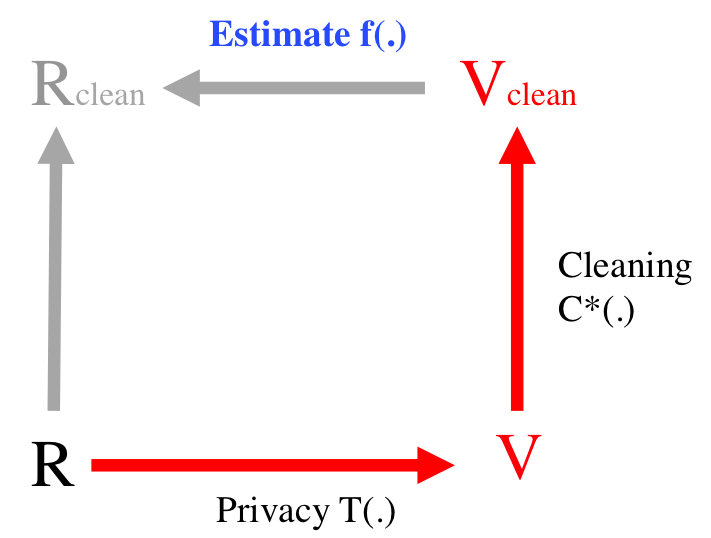
\includegraphics[width=0.6\columnwidth]{figs/example2.png}
 \caption{We want to give users the ability to query the private cleaned view while estimating the result if the query and the data cleaning were applied to original relation. \label{example2}}
\end{figure}

\subsection{Goals of \sys}
Figure \ref{example2} illustrates the primary goal of this work.
A trusted curator applies a randomized transformation $T(\cdot)$ to a dirty relation $R$.
We assume that while the local cleaners are not known to the curator, she does know the partition over discrete attribute values $\{g_1,...,g_k\}$.
The result is a private view $V$.
The untrusted user applies local cleaners to $V$ resulting in $V_{clean}$.
Given an aggregate query $f$ and $V_{clean}$, the goal is to estimate the result of $f(R_{clean})$.
Of course, since the privacy is randomized this estimate is a random variable.
The goal of this work is to present an initial set of analyses about variance and the possibility of the estimate (ultimately related to accuracy).

\noindent We present analysis about the following properties:

\vspace{0.5em}

\noindent\textbf{$\alpha$-error detectability: } Let $r[d]$ be a dirty attribute value, then with probability $1-\alpha$ there exists a record $v \in V$ with the value $r[d]$. Intuitively, this means that an error can be detected with failure rate $\alpha$ over all possible randomized instances of the private view.

\vspace{0.5em}

\noindent\textbf{Unbiasedness: } Let $\hat{q}$ ~ be an estimate of $f(R_{clean})$ based on $V_{clean}$. Unbiasedness means that the expectation of $\mathbf{E}[\hat{q}]$ over all possible randomizations is the true value $f(R_{clean})$.

\vspace{0.5em}

\noindent\textbf{$\alpha$ confidence interval: } Let $\hat{q}$ be an estimate of $f(R_{clean})$. We want a confidence interval of $\pm \delta$ with probability $1-\alpha$. This represents the probability that the estimate deviates from the true value by more than $\delta$.

\begin{example}
A user receives a private view $V$ of the course evaluations, and she wants to count the number of engineering students that responded to the survey.  
She applies an extract operation that finds the phrase ``Engineering" in the \textsf{major} attribute, and runs the SQL query.
\sys estimates the number of engineering students in the original relation.
\end{example}

